% !TEX encoding = UTF-8 Unicode
\chapter{Grundlagen zu auftragsbezogenen Instandhaltungsprozessen}
\markboth{2 Grundlegende Begriffe}{}
\setcounter{footnote}{4}  %um durchgehende Fußnotennummerierung zu haben, hier die Anzahl der bisherigen Fußnoten eintragen

\section{Einordnung in die Produktionswirtschaft und die Begriffsbestimmung}

Unter auftragsbezogenen Instandhaltungsprozessen (engl. maintenance-repair-and\-overhaul (MRO)) wird in dieser Arbeit als ein nachgelagerter Prozess einer erweiterten Leistungserstellung verstanden und ist ein Teilsystem eines Unternehmens, welches den gesamten Wertschöpfungsprozess verlängert. Es handelt sich nicht um die interne oder beauftragte Instandhaltung von u. a. technischen Systemen, sondern um eine Erweiterung des Produktionsprogramms eines Unternehmens. Im weiteren Verlauf dieser Arbeit wird daher von MRO-Prozessen gesprochen. Da es bei MRO-Prozessen um eine Produktion einer Leistung handelt, werden diese der betriebswirtschaftlichen Betrachtung der Produktionswirtschaft zugeordnet.

Bei dem Begriff der Produktionswirtschaft handelt sich um ein Teilgebiet der Betriebswirtschaftslehre.\footnote{Neben der Teilgebiete Finanzwirtschaft, Marketing, Unternehmensführung, Unternehmensrechnung etc., vgl. dazu \cite{Dyckhoff2010}, S. 3.} In der Produktionswirtschaft wird der Fokus auf die Produktion von Leistung gelegt. Bei diesem ökonomischen Konzept wird die Transformation von materiellen und nichtmateriellen Inputgütern (Produktionsfaktoren) hin zu gewünschten Outputgütern (Leistung des Unternehmens) betrachtet. Bei den im Laufe der Zeit erweiterten betriebswirtschaftlichen Produktionsfaktoren nach \citet[S. 71]{Gutenberg:1959aa} handelt es sich um die Elementarfaktoren Werkstoffe, Betriebsstoffe, Betriebsmittel und objektezogene humane Arbeitsleistung sowie um die dispositiven Faktoren Betriebsführung, Organisation und Planung.\footnote{????} Bei Outputgütern handelt es sich um Produkte in Form von Sach- oder Dienstleistungen die dem Markt und somit der potentiellen Nachfrage der Marktteilnehmer zur Verfügung gestellt werden.\footnote{Vgl. \cite{Schmidt:2012aa}, S. 1.} Die Transformation erfolgt durch bestimmte von Menschen veranlasste unternehmerischen Verfahrensweisen.\footnote{Vgl. \cite{tempelmeier1994produktion}, S. 6, echt?????} Beispielsweise kann hier die industrielle Fertigung von Verbrauchs- oder Gebrauchsgütern genannt werden.

Bei der Transformation der Inputgüter erfolgt eine qualitative, quantitative, räumliche oder zeitlichen Veränderung der Objekte.\footnote{Vgl. \cite{Dyckhoff2010}, S. 3.} Durch diese Veränderung kann seitens des Unternehmens eine Leistung auf dem Markt angeboten werden. Damit diese Leistung den Absatz bei potentiellen Konsumenten findet, muss die Leistung durch die Transformation eine Wertschöpfung erhalten. Der konzeptionelle Rahmen dieses Gedankens bildet die Wertschöpfungslehre (engl. suppy chain management (SCM)).\footnote{Vgl. \cite{???}, S. ??.} Danach sollte das Ziel eines jeden Unternehmens das Betreiben von Wertschöpfung sein.\footnote{Vgl. \cite{???}, S. ??.} In der klassischen Auffassung der Wertschöpfungslehre durchläuft die Leistungserstellung alle (Teil-)Systeme des Unternehmens.\footnote{???} Abbildung \ref{Prozess} zeigt in Teil a eine mögliche Abfolge der Systeme eines Unternehmens. Eine klassische Abfolge zur Leistungserstellung bzw. der Transformation von Inputgütern hin zu Outputgütern ist die Abfolge der Systeme Forschung/Entwicklung, Beschaffung, Produktion, Distribution sowie Verkauf. Damit ist die um die Wertschöpfung erhöhte Leistung auf dem Markt angekommen und das Unternehmen erzielt damit i. d. R. einen Ertrag.

\begin{figure}[h!]
  \begin{center}
    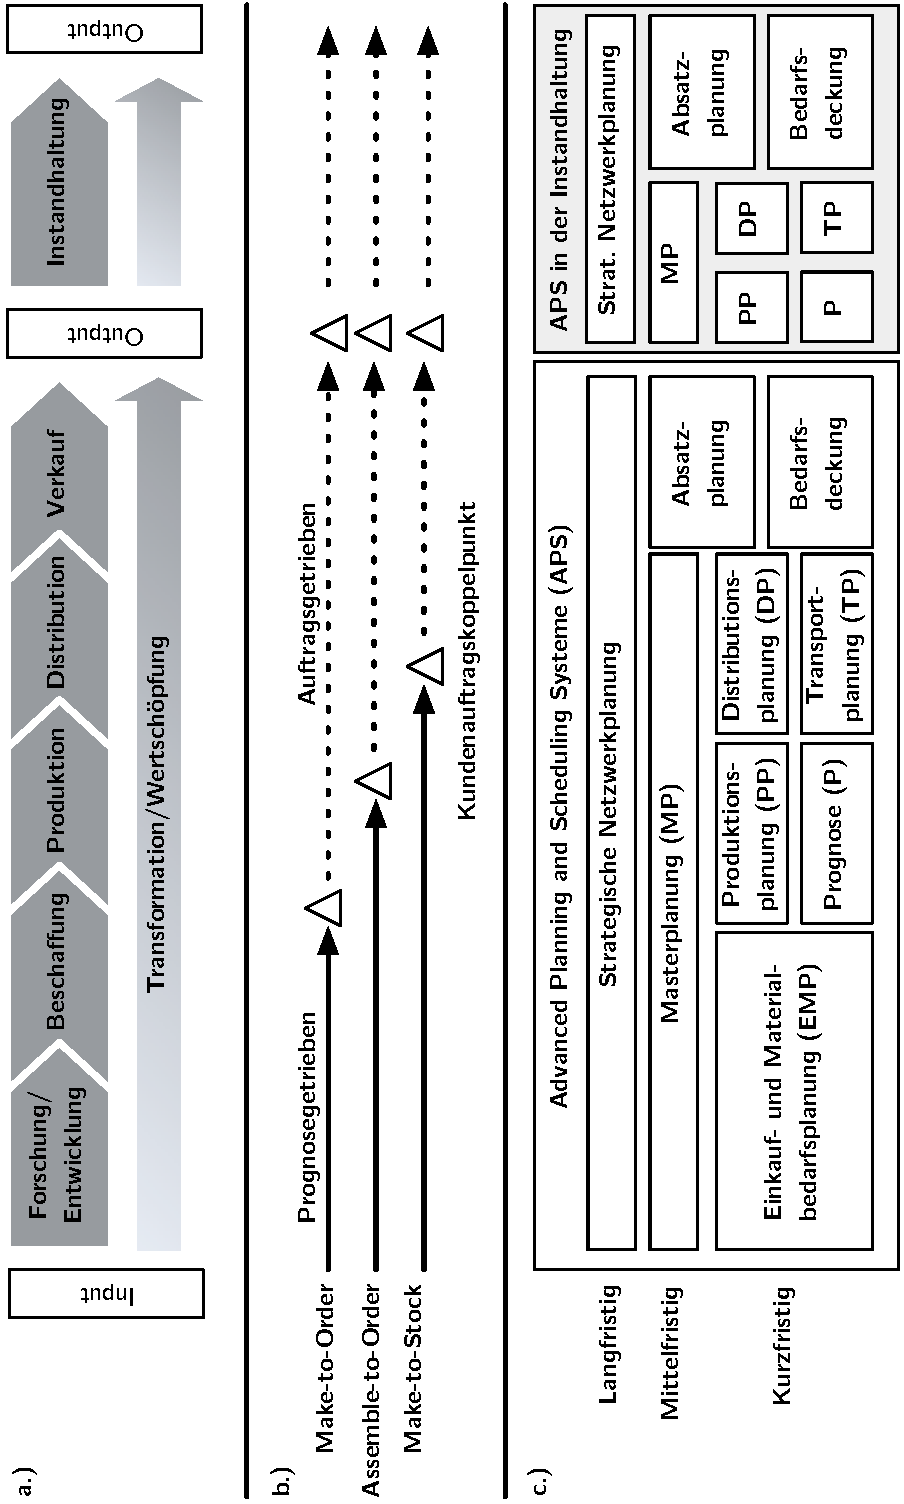
\includegraphics[width=120mm]{Bilder/prozess.pdf}
    \caption{Grafische Veranschaulichung eines Wertschöpfungsprozesses}  \label{Prozess}
    {\footnotesize \textbf{In Anlehnung an:} \cite{Bach:2012aa}, S. 4-5; \cite{quante2009management}, S. 21-22; \cite{meyr2015structure}, S. 100}
  \end{center}
\end{figure}

Sofern das Unternehmen eine \textbf{Instandhaltung} bzw. einen MRO-Prozess als Leistungen anbieten kann, wird die Abfolge des Wertschöpfungsprozesses um dieses Unternehmenssystem erweitert. Für den gewerblichen Verkauf von Gütern an Privatkunden können gesetzliche Regelungen bestehen, womit ein Unternehmen gezwungen ist das Unternehmenssystem der Instandhaltung in den Wertschöpfungsprozess aufzunehmen.\footnote{Vgl. die Richtlinie 1999/44/EG des Europäischen Parlaments und des Rates vom 25. Mai 1999 zu bestimmten Aspekten des Verbrauchsgüterkaufs und der Garantien für Verbrauchsgüter.} Anderseits kann ein Unternehmen auch die Instandhaltung seiner eigenen Güter als eigenständig angebotene Leistung bereitstellen und damit den Gesamtertrag des Unternehmens erhöhen (MRO-Prozess). Dieses wird oft von Unternehmen angeboten, die ihren Umsatz mit komplexen Produkten erzielen. Komplexe Produkte zeichnen sich durch ihre hohe Anzahl an hochtechnologischen Komponenten aus, die erst durch den vollständigen und meist kostenintensiven Zusammenschluss eine individuelle Bedürfnisbefriedigung des Nachfragers ermöglichen.\footnote{Vgl. \cite{komplexe2009Schmidt}, S. 97} In dieser Arbeit werden solche komplexen Produkte betrachtet, die aus einer Vielzahl von Komponenten bzw. Ressourcen bestehen.

\citeauthor{helbing2010instandhaltung} versteht unter Instandhaltung die \glqq Gesamtheit der technischen und organisatorischen Mittel, Vorgänge und Maßnahmen zur Erhaltung, Verbesserung und Wiederherstellung des Funktions-, Leistungs- und Güteniveaus von materiellen Objekten während ihrer Wirkungs- und Lebenszeit durch Wartung, Inspektion und Instandsetzung.\grqq\footnote{Vgl. \citeauthor{helbing2010instandhaltung}, S. 984} In dieser Arbeit ist mit dem Begriff der MRO-Prozesse gemeint, dass für die betrachteten komplexen Produkte ein spezifischer Ausführungsmodus für die Anfragen verwendet wird, der eine erneute Integration von produkt-spezifischen Ressourcen vorsieht, damit die Funktionsfähigkeit des Produkts (Leistung) wiederhergestellt ist. Damit lässt sich das Verständnis des Begriffs als Leistung eines Unternehmens und als Unternehmenssystem ableiten, welches die Verlängerung und zugleich als Erweiterung des Wertschöpfungsprozesses versteht.

\section{Charakteristika}

Nach der DIN 310511 wird Instandhaltung insofern ausgeführt, wenn die Funktionsfähigkeit Betrachtungseinheit sichergestellt werden muss, damit der ursprüngliche Wert erhalten bleibt.\footnote{Vgl. \cite{Strunz:2012aa}, S. 1.} Betrachtungseinheit können ganze Anlagen und Maschinen sein oder nur einzelne Komponenten.\footnote{Vgl. \cite{schenk2010techSys}, S. 23.}

Erläuterung nach DIN 31051:\footnote{Unbedingt nachlesen!!!!}
\begin{itemize}
\item Instandhaltung ist die Kombination aller technischen und administrativen Maßnahmen des Managements während des Lebenszyklus einer Betrachtungseinheit zur Erhaltung des funktionsfähigen Zustandes oder der Rückführung in diesen, so dass sie die geforderte Funktion erfüllen kann.
\item Als Betrachtungseinheit (BE) wird jedes Bauelement, Gerät, Teilsystem, jede Funktionseinheit, jedes Betriebsmittel oder System, das für sich allein betrachtet werden kann, definiert.
\end{itemize}

Nach der DIN 31051 werden Einheiten betrachtet, die eine Wartung, Inspektion, Instandsetzung oder Verbesserung bedürfen.\footnote{Vgl. \cite{schenk2010techSys}, S. 23-24} Bei einer Wartung handelt es sich um Maßnahmen zur Verzögerung der Abnutzung. Die Inspektion umfasst alle Maßnahmen der Begutachtung sowie der Beurteilung des Ist-Zustandes einer Betrachtungseinheit und die Instandsetzung beinhaltet die Maßnahmen zur Wiederherstellung des Sollzustands. Mit der Verbesserung sind Maßnahmen gemeint, die den Soll-Zustand der Betrachtungseinheit erweitern, damit mögliche Defekte verhindert werden.

Instandhaltungsprozesse lassen sich weiter nach Ausführungszeitpunkte und des Ausführungsorte der Maßnahmen unterscheiden.\footnote{Vgl. \cite{schenk2010techSys}, S. 24-26; \cite{hinsch2010instandhaltung}, S. 190-191} Diese Unterscheidung spielt bei der Betrachtung von MRO-Prozessen eine untergeordnete Rolle. 

Da der Absatz zeitlich vor der Produktion der Leistung stattfindet, handelt es sich bei dem hier betrachteten MRO-Prozessen um eine Auftragsfertigung.\footnote{Vgl. \cite{hax1956industriebetrieb}, S. 247; \cite{Gutenberg1965dispos}, S. 164-165} In der Literatur wird für die Auftragsfertigung oft der englischen Begriff \textit{Make-to-Order (MTO)} verwendet. Abzugrenzen ist der Begriff von der Lagerfertigung (engl. Make-to-Stock (MTS)) und der kundenindividuellen Fertigung mit standardisierten Komponenten (engl. Assemble-to-Order (ATO)). 
Dies kann zum einen anhand des Kundenauftragskoppelpunkt und zum anderen anhand der Planungsgrundlage der Leistungserstellung getätigt werden. Der Kundenauftragskoppelpunkt zeigt den erstmaligen Kundenkontakt bzw. Auftragseingang auf. Mit Eingang des Kundenauftrags wechselt die Planungsgrundlage der Leistungserstellung von prognosegetriebener hin zu auftragsgetriebener Planung. Die prognosegetriebenen Planungsgrundlage für die Fertigung ist mit einem Prognosefehler für die Wiederauffüllung der Ressourcen behaftet, was der analytischen Betrachtung des Kundenauftragskoppelpunkts zur Bestimmung der notwendigen Ressourcenkapazität und der weiteren Auftragseingänge weiteres Gewicht verleiht.\footnote{Vgl. \cite{quante2009management}, S. 21} 

Bei einer MTO trifft vor der eigentlichen Produktion der Leistung der Kundenauftrag ein. Damit sind die Forschungs/Entwicklung der Leistung und die Beschaffung der Komponenten bzw. Ressourcen hauptsächlich prognosegetrieben. Alle weiteren Teilsysteme des Unternehmens können sich speziell an den Forderungen des Auftrags richten. Ähnliche Rahmenbedingung besitzt eine ATO, die den Kundenauftragskoppelpunkt innerhalb des Produktionsablaufs hat. Da nur ein gewissen Umfang der Komponenten an auftragsspezifischen Eigenschaften angepasst wird, sind die Grundkomponenten der Produkte abhängig der Prognosemethoden des Unternehmens. Bei MTS erfolgt der Auftragseingang erst nach der Produktion, womit diese Fertigungsart den höchsten Anteil des Einsatzes von Prognosemethoden aufweist.\footnote{Vgl. \cite{fleischmeyr2004codp}, S. 300-303; \cite{quante2009management}, S. 21-22} Abbildung \ref{Prozess} zeigt im Teil b die Unterschiede der Fertigungsarten im Verlauf des Wertschöpfungsprozesses. 

Da bei MRO-Prozessen erst mit Auftragseingang die erforderlichen Produktionsschritte und der Ressourcenbedarf bekannt sind, werden diese mit MTO-Prozessen gleichgesetzt. Zur Erfüllung möglichst vieler Aufträge muss eine möglichst gute Prognose der benötigen Ressourcen vorliegen, damit kurze Liefer- und Durchlaufzeiten gewährleistet bleiben.\footnote{Vgl. \cite{thaler2001supply}, S. 68.} Sofern die Prognose fehlerhaft ist und ein zu geringer Bestand an Ressourcen vorhanden ist, konkurrieren die unterschiedlich eintreffenden Anfragen nach MRO-Prozessen des Unternehmens bzgl. der Ressourcen untereinander. Sofern ein zu hoher Ressourcenbestand vorhanden ist, stellt sich die Frage über den besten Mix der unterschiedlichen Aufträge, damit die Ressourcenkapazität optimal genutzt wird und dementsprechend der Ertrag maximiert wird. Im nächsten Abschnitt wird dieser Frage in Bezug von Produktionsplanungssystemen und der betrieblichen Entscheidungsfindung weiter nachgegangen.


\section{Relevanz für betriebliche Entscheidungen}

Die Entscheidung über die Ausgestaltung des MRO-Prozesses hat eine hohe Relevanz für den Erfolg der angebotenen Leistung sowie der Effizienz des gesamten SCM-Prozesses des Unternehmens und kann der nachhaltigen Konsumentenzufriedenheit dienen. Wichtiger Erfolgsfaktor für ein erfolgreiches SCM und somit der Konsumentenzufriedenheit ist der Einsatz von Advanced Planning and Scheduling Systemen (APS).\footnote{Vgl. \cite{fleischmeyr2004codp}, S. 298}

Bei APS handelt es sich um computergestützte Systeme, mit denen die Planung der ganzheitlichen Wertschöpfung der Leistung mit Hilfe von mathematischer Modelle des Operations Research (OR) unterstützt wird.\footnote{????? steht eig auch bei Fleischmeyer, aber besser andere Quelle finden...} Neben der reinen Planung der Produktion, helfen moderne APS mit ihrem modularen Aufbau auch bei der gesamten Auftragsabwicklung und unterstützen damit Unternehmensteilnehmer bei betrieblichen Entscheidungen innerhalb des SCM-Prozesses, wie z. B. bei dem Einkauf von Ressourcen, der Produktionsplanung und dem Absatz der Leistung.\footnote{Vgl. \cite{meyr2015structure}, S. 99-100; \cite{fleischmeyr2004codp}, S. 298} \cite{meyr2015structure} sortieren einige wichtige Module eines APS in den Dimensionen des SCM-Prozesses und des Planungshorizonts. Abbildung \ref{Prozess} in Teil c greift diese Sortierung auf. Bei dem Modul der strategischen Netzwerkplanung werden die Lieferanten, Werke und Lagerpunkte in einer langfristigen Betrachtungsweise festgelegt. Die Entscheidungen die Aufgrund der strategischen Netzwerkplanung getroffen werden, haben großen Einfluss auf die langfristige Rentabilität sowie Wettbewerbsposition des Unternehmens und haben räumlichen und zeitlichen Charakter.\footnote{Vgl. \cite{goetschalckx2005strategic}, S. 117-118} D. h. das Unternehmen die Planungsmodelle und Entscheidungen aufgrund der strategischen Netzwerkplanung in Bezug auf bestimmte regionale Gegebenheiten und einem vordefinierten Betrachtungszeitraum festlegen.\footnote{Datengrundlage bilden u. a. Prognosen und Wirtschaftstrends.} Die Absatzplanung dient einerseits der Absatzprognose und anderseits der Analyse der notwendigen Sicherheitsbestände.\footnote{Vgl. \cite{fleischmeyr2004codp}, S. 298, \label{fleisch}} Das Modul Masterplanung synchronisiert den Materialfluss entlang des gesamten SCM-Prozesses und unterstützt dadurch mittelfristige Entscheidungen über die effiziente Nutzung der Ressourcen, damit für einen kontinuierlichen Materialfluss größere Puffer gemieden werden.\footnote{Vgl. \cite{rohde2002scm}, S. 143.} Mit dem Modul der Einkaufs- und Materialbedarfsplanung werden kurzfristig terminierte Pläne für Komponenten und Teile (Ressourcen) für die Fertigung berechnet.\footnote{Vgl. \cite{stadler2008aps}, S. 217-218.} Aufbauend auf diesen Plänen kann die Produktionsplanung und die weitere Prognose für die Produktion und Logistik erfolgen, die den organisatorischen Anforderungen des Produktionssystems gerecht werden müssen und einen kurzfristigen Planungshorizont aufweisen.\footref{fleisch} Bei diesen Modulen werden in einer kurzfristigen Betrachtung u. a. die Maschinenverfügbarkeit und die Losgrößen geplant bzw. prognostiziert. Eine effiziente Produktionsplanung setzt eine gute Prognose voraus.\footnote{Vgl. \cite{dickersback2004pp}, S. 131.} Bei den Modulen der Distributions- und Transportplanungen werden die Pläne für die Verkaufsstellen und die Logistik generiert.\footref{fleisch} Zum Abschluss wird das Modul Bedarfsdeckung aufgeführt. Das Modul dient hauptsächlich der Kundenzufriedenheit, indem es die eintreffenden Kundenaufträge auf Realisierbarkeit prüft und die geforderte Lieferung der Leistung zusagt.\footref{fleisch}

Diese Module wurden von \cite{meyr2015structure} jedoch im Verhältnis eines typischen SCM-Prozess gesetzt. Es stellt sich die Frage, welche Systeme bei betriebliche Entscheidungen durch Einbeziehung von MRO-Prozessen in den SCM-Prozess relevant sind. Die strategische Netzwerkplanung scheint keinen Einfluss auf MRO-Prozesse zu haben, da diese sich an der Grundleistung des Unternehmens orientiert. Anders formuliert bedeutet dies, dass nur dort eine Instandhaltung der Produkte angeboten wird, wo auch das eigentliche Produkt den Absatz findet. Inwieweit die Masterplanung ebenfalls den Materialfluss von MRO-Prozessen synchronisiert wird in dieser Arbeit nicht betrachtet. Die Distributionsplanung findet keine Relevanz bei MRO-Prozessen, da es sich um Auftragsfertigung handelt.

Bei MRO-Prozessen sind die Module der Absatzplanung, der Einkaufs- und Materialbedarfsplanung, der Produktionsplanung, die Transportplanung und der Bedarfsdeckung relevant. Ein effizientes APS bei MRO-Prozessen muss den erwarteten Absatz bzw. die erwarteten Auftragseingänge mittelfristig gut prognostizieren können. Aufbauend auf dieser Prognose kann eine Einkaufs- und Materialbedarfsplanung erfolgen. Dies erfolgt jedoch kurzfristig, da der Ressourcenbedarf abhängig der Kundenaufträge ist. Anschließend erfolgt bereits die Prüfung der Realisierbarkeit und abhängig dieser die Entscheidung über die Annahme des Auftrags über die Instandsetzung des Produkts mittels des Moduls der Bedarfsdeckung. Anschließend erfolgt die Produktions- und Transportplanung.

In dieser Arbeit wird der Fokus auf die Auftragsannahme mittels des Moduls der Bedarfsdeckung gelegt. Die Entscheidung, ob ein Auftrag zur Instandhaltung angenommen wird, ist abhängig der verfügbaren Ressourcenkapazität und des Lagerbestand an Teilen bzw. Fertigerzeugnissen (Produkten). %Hier muss eine Differenzierung der Begriffe Ressourcenkapazität und Lagerbestand erfolgen.
Mit Ressourcenkapazität wird in dieser Arbeit ein Bestand an den Produktionsfaktoren Produktionskapazität oder Arbeitskraft verstanden. Es handelt sich hier um erneuerbare Ressourcen, die mit Ablauf des Betrachtungszeitraums den vordefinierten Kapazitätswert wieder annehmen. Bei dem Lagerbestand handelt es sich um einen physischen Bestand an Teilen, die für die Fertigung bzw. Instandhaltung verwendet werden, oder um Fertigerzeugnisse. Fertigerzeugnisse sind die durch den Fertigungsprozess erzeugten Leistungen in Form von Produkten. Für die Entscheidungsträger muss das Modul der Bedarfsdeckung dementsprechend die Entscheidung über die Auftragsannahme unter Beachtung der Auftrags-, der Materialbedarfs- und der Produktionsplanung unterstützen. Im nächsten Kapitel wird eine OR-Methode zur klassischen Auftragsannahme bei konstanten Ressourcenkapazitäten vorgestellt und im Kapitel \ref{???} wird dieses Modell um die Besonderheiten der MRO-Prozesse erweitert.





